The goal was to estimate joint torques \comment{which are dynamically consistent}{Ceci est vrai en permanence, pas besoin de le mentionner je pense (dans le cas d'un article dédié à la marche peut-être, mais ici, ça l'est par définition)} during one gait cycle from the first heel strike to the end of the swing phase using a 3D one-leg torque driven model with 12 DoFs.  \\

\comment{The experimental joint angles}{Donc c'est du tracking? Il faut le dire dans le paragraphe précédent} \comment{$q_m$}{$q_p$ n'a pas été déclaré, ni les \omega, ni OC} (obtained from markers using an extended Kalman filter), ground reaction forces $F_m$ and moments \comment{$M_m$}{Pas la même nomenclature que dans l'équation} were \comment{tracked}{Ah! Je ne vois pas le but de faire deux paragraphes alors}:

\begin{eqnarray}
\label{eq:ocp_q}
\mathcal{J} = \sum_{i=1}^{N_i}\Bigg(\underbrace{\omega_1(\|q_p - q_m\|^{2})}_{TRACK\_STATE}
\label{eq:ocp_forces}
\end{eqnarray}
\begin{eqnarray}
+ \underbrace{\omega_2(\|\sum_{c=1}^{N_c}F_c - F_m\|^{2})}_{TRACK\_FORCES}
\end{eqnarray}
\begin{eqnarray}
\label{eq:ocp_moments}
+ \underbrace{\omega_3(\|\sum_{c=1}^{N_c}OC\times F_c - M_{m,O}\|^{2})}_{TRACK\_MOMENTS}\bigg) 
\end{eqnarray}

\noindent where $N_i$ and $N_c$ are the number of time frames and contact points, respectively. 

The interaction between the ground and the foot was modelled using a 4-contact \comment{point}{points?} model located at the heel and the forefoot (first and fifth metatarsi and toes - digit of the second toe). 
The stance phase was divided in three to follow the natural rolling movement of the foot from heel strike to toe off: heel, flatfoot and forefoot contacts. 
A constraint of \comment{non-slipping}{Dire ce que ça fait, sinon c'est trop obscur} (NON\_SLIPPING) and \comment{unilateral contact force}{Dire ce que ça fait, sinon c'est trop obscur} (CONTACT\_FORCE) were added for each stance phase. 
The use of the IMPACT state transition allowed to represent the gain of contact(s) from a system without any contact (swing phase) to a system with contacts (heel strike) [\addref\ thesis Felis - articles?].  


Based on force plateform data and markers position, each phase had a definite time inducing a complete simulation time of 0.93 s and was discretized in 94 intervals. 
The solution was able to reproduce a complete gait cycle [value RMSE - better with 3 contact points?] (Fig.~\ref{fig:snapshots_multiphase_walking_cycle}). 

\begin{figure*}[t!]
\centering
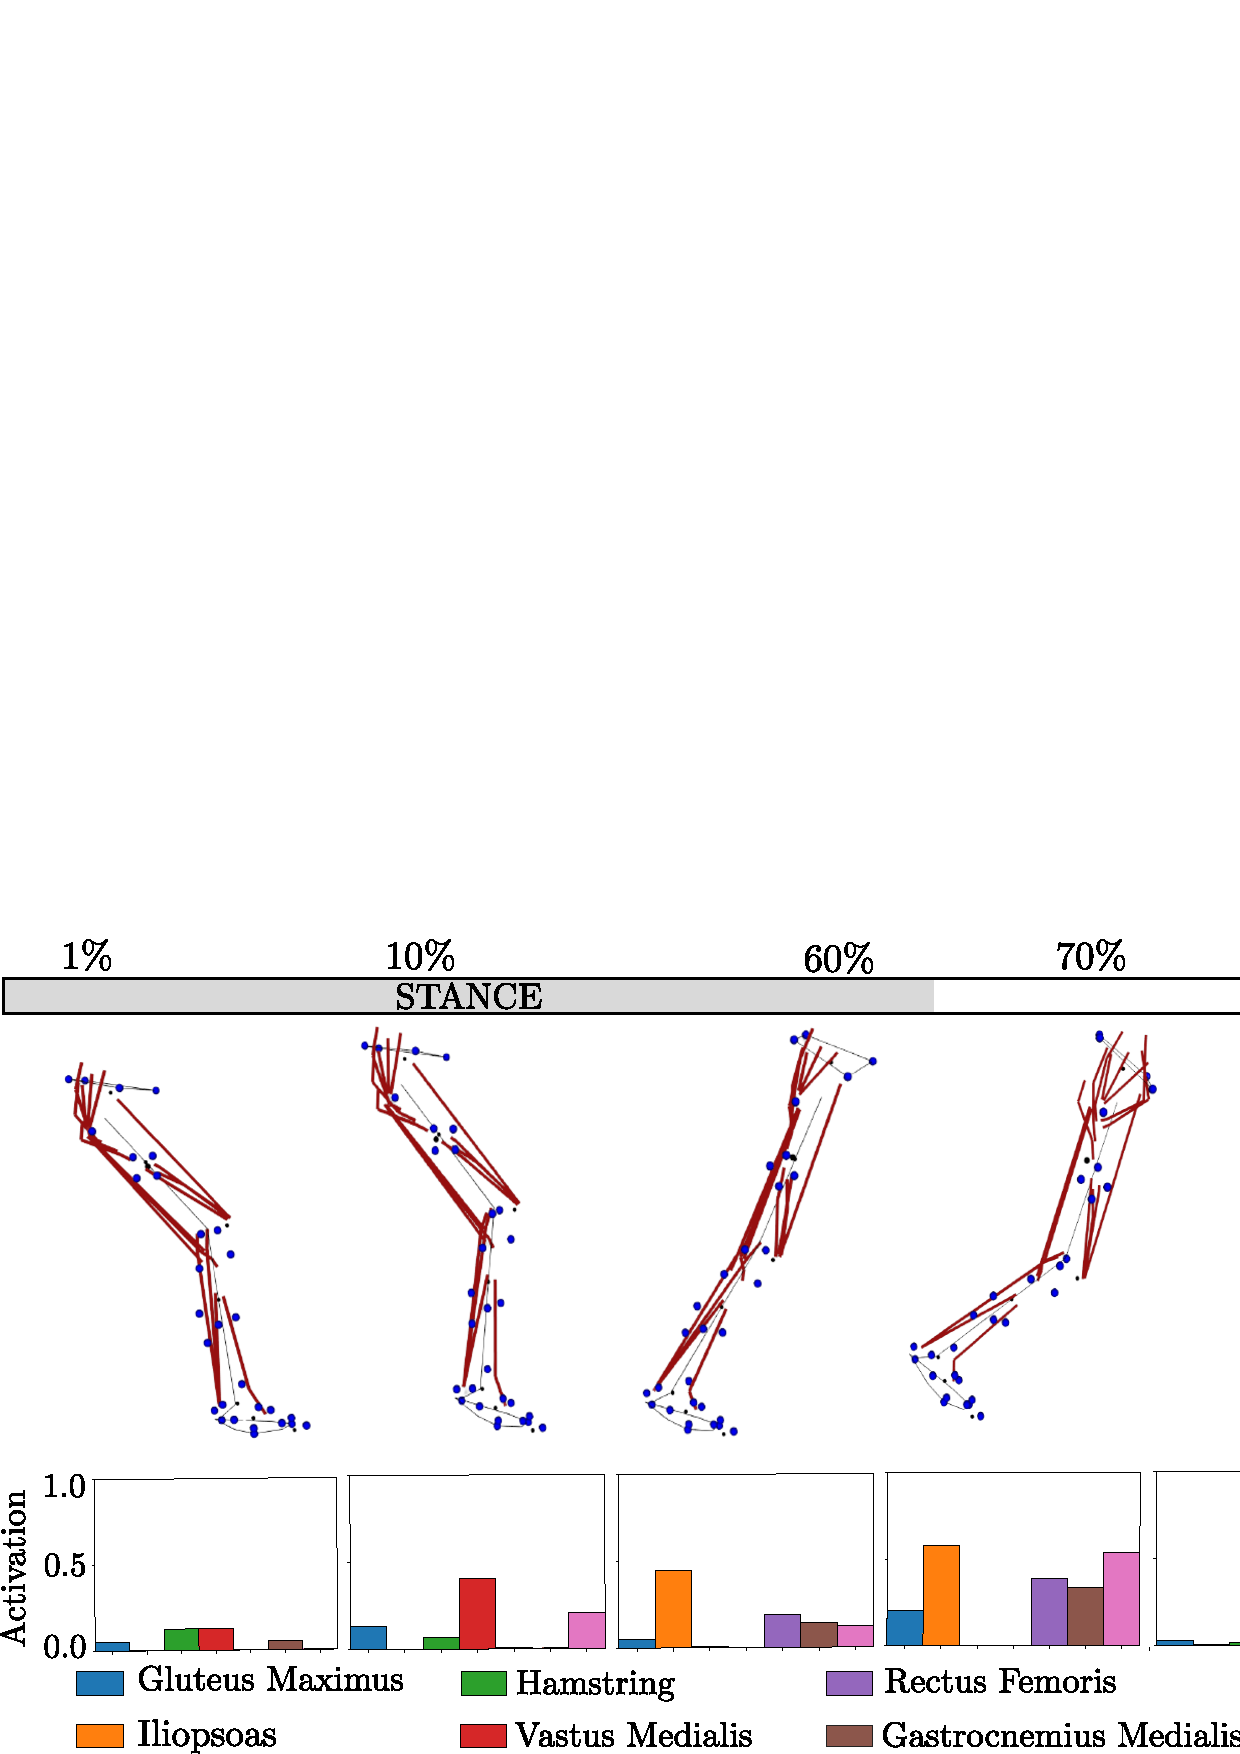
\includegraphics[width=\textwidth]{figures/multiphase_walking_cycle.png}\\
\caption{Snapshots of a walking gait cycle driven by torque actuators.}
\label{fig:snapshots_multiphase_walking_cycle}
\end{figure*}

%\begin{table}[h!]
%\caption{\small Objective terms of the Multiphase torque driven walking cycle }
%\label{tab:Multiphase_torque_driven_walking_cycle}
%\centering
%\begin{tabular}{c c c c}
%\toprule 
%& Type & Function & Weight \\ 
%\midrule
%$\#1$ & Lagrange & TRACK\_ STATE & $1e5$ \\ 
%\midrule
%$\#2$ & Lagrange & MINIMIZE\_ TORQUE\_ DERIVATIVE & $1e-2$ \\ 
%\midrule
%$\#3$ & Lagrange & TRACK\_ GRF & $1e-2$ \\ 
%\midrule
%$\#4$ & Lagrange & TRACK\_ MOMENTS & $1e-1$ \\
%\bottomrule
%\end{tabular}
%\end{table}
